\documentclass[12pt, oneside]{book}
\usepackage{newtxtext,newtxmath}
% \usepackage{mathptmx}


\usepackage[a4paper, top=3cm, left=3cm, bottom=2.5cm, right=2.5cm]{geometry}

\usepackage[utf8]{inputenc}
\usepackage[toc]{glossaries}

\usepackage{ktustyle}

\usepackage[nottoc, numbib]{tocbibind}

\usepackage[sorting=none]{biblatex} 
\addbibresource{References.bib}

\usepackage{fancyhdr}


\usepackage{caption}

\captionsetup{
  font=footnotesize,
  justification=raggedright,
  singlelinecheck=false
}

\begin{document}


\begin{titlepage}
    \begin{center}
    
        \textbf{\KTU \\ \titleFac}
        \vspace*{3cm}
        
            \centering
            \textbf{\anabilim}
            
        \vspace*{1.5cm}
        
            \centering
            \textbf{\titleOfThesis}
        \vspace*{2.5cm}
        
            \centering
            \textbf{\seminer}
    \end{center}
        
        \vspace{2cm}
        
        \hspace{1cm}{
            \textbf{\studentName \hspace{1cm}{:} \hspace{0.5cm}{\studentNameFill}}} 
            
        \hspace{1cm}{    
            \textbf{\studentNumber \hspace{3cm}{:} \hspace{0.5cm}{\studentNumberFill}}}
        
        \vspace{1cm}
        
        \hspace{1cm}{    
            \textbf{\advisorT \hspace{3.2cm}{:} \hspace{0.5cm}{\advisorTFill}}}
        
        \vspace{2cm}
        
        \hspace{1cm}{    
            \textbf{\PresentationDate \hspace{1cm}{:} \hspace{0.5cm}{{\PresentationDateFill}}}}


\end{titlepage}
\pagenumbering{Roman}
\newcommand\CentChapters{
  \titleformat{\chapter}[display]
  {\normalfont\bfseries\normalsize\centering}{\thesection}{1em}{\MakeUppercase}
}
\CentChapters


\makeatletter
% \patchcmd{<cmd>}{<search>}{<replace>}{<succes>}{<failure>}
\patchcmd{\@chapter}{\addtocontents{lof}{\protect\addvspace{10\p@}}}{}{}{} %figüre chapter aralıkları
\patchcmd{\@chapter}{\addtocontents{lot}{\protect\addvspace{10\p@}}}{}{}{}% tablo chapter aralıkları




%%%%Table of Contents%%%%

\setstretch{1}
\newcommand*{\disableboldchapterintoc}{%
  \addtocontents{toc}{\string\renewcommand{\protect\cftchappagefont}{\protect\normalfont}}
  \addtocontents{toc}{\string\renewcommand{\protect\cftchapfont}{\protect\normalfont}}
  \addtocontents{toc}{\string\renewcommand{\protect\cftchapleader}{\protect\normalfont\protect\cftdotfill{\protect\cftsecdotsep}}}% 
}


\newcommand{\addchapscorerule}{\addtocontents{toc}{\protect\chapruletrue}}


\renewcommand{\cftdotsep}{1}
\renewcommand{\cftchapleader}{\cftdotfill{\cftsecdotsep}}% dot leaders in bold
\renewcommand{\contentsname}{\hfill\bfseries\large  \content \hfill}
\addtocontents{toc}{\protect{}{\hspace*{\fill} \textbf{\underline{Sayfa No}}}} % Write the header line

\addtocontents{toc}{\vskip0.5\baselineskip\par}% Some vertical spacing 

% \addtocontents{toc}{\setcounter{tocdepth}{2}} en fazla derinlik 2 olması için


\disableboldchapterintoc
\renewcommand\cftchapaftersnum{.\hfill}
\renewcommand{\cftsecaftersnum}{.\hfill}
\renewcommand{\cftsubsecaftersnum}{.\hfill}

% section ve subsectionları chapter ile aynı hizaya alır
\cftsetindents{chapter}{0em}{4em}
\cftsetindents{section}{0em} {4em}
\cftsetindents{subsection}{0em}{4em}
% chapterlardaki önceki boşluk
\setlength{\cftbeforechapskip}{0.5em}

\setstretch{1.5}
\setlength{\parindent}{1cm}
\chapter*{ÖNSÖZ}

Bu çalışmada plevral efüzyon sitopatolojik görüntülerin derin öğrenme yöntemiyle
otomatik algılanması sağlanmıştır. Veri tabanı hazırlama sürecinde ise görüntüler mikroskoptan
okunarak panorama yöntemiyle birleştirilmiştir ve bu görüntüden belirli boyutlarda görüntüler
kesilerek hazırlanması sağlanmıştır. Bu çalışmada danışmanlığımı üstlenen değerli hocam Dr. Öğr. Üyesi Murat AYKUT'a ilgi, destek ve tecrübelerinden dolayı teşekkürü bir borç bilirim.
Çalışmam boyunca bana her türlü desteği sağlayan yüksek
lisans eğitimim boyunca sabır, destek ve sevgileriyle yanımda olan aileme ve dostlarıma çok
teşekkür ederim.

\vspace{1.5cm}
\hfill Murat Can VARER

\hfill Trabzon 2021

\addcontentsline{toc}{chapter}{ÖNSÖZ}
\chapter*{TEZ ETİK BEYANNAMESİ}
    Yüksek Lisans Tezi olarak sunduğum HİPERSPEKTRAL UYDU GÖRÜNTÜLERİNİN SINIFLANDIRILMASINDA VAE VE CNN İLE HİBRİT BİR YAKLAŞIM başlıklı bu çalışmayı
baştan sona kadar danışmanım Dr. Öğr. Üyesi Murat AYKUT’un sorumluluğunda
tamamladığımı, verileri/örnekleri kendim topladığımı, deneyleri/analizleri ilgili
laboratuarlarda yaptığımı/yaptırdığımı, başka kaynaklardan aldığım bilgileri metinde ve
kaynakçada eksiksiz olarak gösterdiğimi, çalışma sürecinde bilimsel araştırma ve etik
kurallara uygun olarak davrandığımı ve aksinin ortaya çıkması durumunda her türlü yasal
sonucu kabul ettiğimi beyan ederim. 28/05/2021

\vspace{1.5cm}
\hfill Murat Can VARER

\addcontentsline{toc}{chapter}{TEZ ETİK BEYANNAMESİ}

\setstretch{1}
\tableofcontents


\chapter*{\normalfont Yüksek Lisans Tezi}


\begin{center}
\vspace{-1.2cm}
    ÖZET\\
    \vspace{0.33cm}
    HİPERSPEKTRAL UYDU GÖRÜNTÜLERİNİN SINIFLANDIRILMASINDA\\ VAE VE CNN İLE HİBRİT BİR YAKLAŞIM\\
    \vspace{0.33cm}
    Murat Can VARER\\
    \vspace{0.33cm}
    \setstretch{1}
    Karadeniz Teknik Üniversitesi\\
    Fen Bilimleri Enstitüsi\\
    Bilgisayar Mühendisliği Anabilim Dalı\\
    Danışman: Dr. Öğr. Üyesi Murat AYKUT
\end{center}
\vspace{0.5cm}
\setstretch{1.5}
Yüksek hesaplamaların daha hızlı yapıldığı günümüz teknolojisinde artık işlem yükü fazla olan projeler daha kolaylıkla yapılmaktadır. Evrişimsel sinir ağları (ESA) (Convolution Neural Networks (CNN) ) görüntüler için sınıflandırma problemlerini çözmek amaçlı geliştirilmiş bir Derin öğrenme modelidir.
Derin öğrenme, öğrenme düzeylerini temsil eden makine öğrenmesinin dalını ifade eder yani burada bahsi geçen derin kelimesi, sınıflandırılacak görüntülerin özelliklerini sinir ağı yapısının derinliğinden alır. Varyasyonel Oto-Kodlayıcı (VOK) (Variational AutoEncoder (VAE) ), temelde danışmansız öğrenme olarak kullanılan bir yöntemdir. Amaç görüntülerin boyutu küçülterek daha farklı görüntülerin elde edilmesi için gizli katman adı verilen alanda Gaussian gürültüsü uygulayarak temelde çeşitliliği arttırmaktır. 

Uzaktan algılama, dünyanın yüzeyi hakkında bilgi edinme bilimidir. Günümüzde uzaktan algılama başta askeri hava sahası olmak üzere deprem hazırlığı aşamasında toplanma bölgelerinin de belirlenmesinde önemli rol oynamaktadır. Bu tez çalışmasında uydudan çekilmiş Hiperspektral Görüntüleri (Hyperspectral İmages (HSI) ) CNN modelini kullanarak sınıflandırılması yapılacaktır.
\\
\\
\textbf{Anahtar Kelimeler}: Evrişimsel Sinir Ağları, Varyasyonel Oto-Kodlayıcı, Derin Öğrenme, 

                            \hspace{2.7cm}Uzaktan Algılama

\addcontentsline{toc}{chapter}{ÖZET}
\chapter*{ \normalfont Master Thesis}

\begin{center}
    \vspace{-1.25cm}
    SUMMARY\\
    \vspace{0.33cm}
    A HYBRID APPROACH TO THE CLASSIFICATION OF HYPERSPECTRAL SATELLITE IMAGES VAE AND CNN \\
    \vspace{0.33cm}
    Murat Can VARER\\
    \vspace{0.33cm}
    \setstretch{1}
    Karadeniz Technical University\\
    The Graduate School of Natural and Applied Sciences\\
    Computer Engineering Graduate Program\\ 
    Supervisor: Asst. Prof. Murat AYKUT
\end{center}
\vspace{0.5cm}
\setstretch{1.5}
In today's technology, where high calculations are made faster, projects with high processing load can be done more easily. Convolutional neural networks (ESA) (Convolution Neural Networks (CNN)) is a Deep learning model developed to solve classification problems for images.
Deep learning refers to the branch of machine learning that represents levels of learning, so the word deep referred to here derives the properties of the images to be classified from the depth of the neural network structure.The Variational AutoEncoder (VAE) is basically a method used as unsolicited learning. The aim is to increase the variety by applying Gaussian noise in the area called the hidden layer in order to obtain more different images by reducing the size of the images.

Remote sensing is the science of obtaining information about the earth's surface. Nowadays, remote sensing plays an important role in determining the gathering areas during the earthquake preparation phase, especially in military airspace. In this thesis, Hyperspectral Images (HSI) taken from satellite will be classified using CNN model.
\\
\\
\textbf{Key Words}: Convolution Neural Networks, Variational AutoEncoder, Deep Learning,


                    \hspace{1.12cm} Remote Sensing

\addcontentsline{toc}{chapter}{SUMMARY}





%%%%%%%%%%%%%%%%%%%%%%%%%%%%%%%%%%%%%%%%%%%%%%%%%%%%%%%%
%%%%%%%%%%%%%%%%%%%%%%%%%%%%%%%%%%%%%%%%%%%%%%%%%%%%%%%%
%%%%%%    TABLO, ŞEKİL     %%%%%%
%%%%%%%%%%%%%%%%%%%%%%%%%%%%%%%%%%%%%%%%%%%%%%%%%%%%%%%%
%%%%%%%%%%%%%%%%%%%%%%%%%%%%%%%%%%%%%%%%%%%%%%%%%%%%%%%%
\setstretch{1.5}
\newlength{\mylen }
\newlength{\tempp }
\setlength{\tempp}{\cftfignumwidth}

\newpage

\renewcommand{\figurename}{\figureName }
\renewcommand{\cftfigpresnum}{\figurename }
\renewcommand{\cftfigaftersnum}{}
\settowidth{\mylen}{\cftfigpresnum\cftfigaftersnum}
\addtolength{\cftfignumwidth}{\mylen}
\addtocontents{lof}{\protect{}{\hspace*{\fill} \textbf{\underline{Sayfa No}}}} % Write the header line
\addtocontents{lof}{\vskip0.5\baselineskip\par}% Some vertical spacing 
\renewcommand{\listfigurename }{\listfigures }
% \let\origaddvspace\addvspace
% \renewcommand{\addvspace}[1]{}
\listoffigures
\newpage
\renewcommand{\tablename}{\tableName }
\renewcommand{\cfttabpresnum}{\tablename }
\renewcommand{\cfttabaftersnum}{}
\settowidth{\mylen}{\cfttabpresnum\cfttabaftersnum}
\addtolength{\cfttabnumwidth}{\mylen}


\renewcommand{\cftloftitlefont}{\hspace*{\fill}\Huge\bfseries}
\renewcommand{\cftafterloftitle}{\hspace*{\fill}}
\renewcommand{\listtablename}{\listtables}
\addtocontents{lot}{\protect{}{\hspace*{\fill} \textbf{\underline{Sayfa No}}}} % Write the header line
\addtocontents{lot}{\vskip1\baselineskip\par}% Some vertical spacing 

\listoftables

\input{Chapters/kısaltmalar}

\clearpage


\titleformat{\chapter}
  {\normalfont\normalsize\bfseries}{\thechapter.}{1em}{}
\titlespacing{\chapter}{1cm}{\myonehalfvspace plus 4pt minus 2pt}{\myonehalfvspace plus 2pt minus 2pt}
% Section heading
\titleformat{\section}
  {\normalfont\normalsize\bfseries}{\thesection.}{.5em}{}
\titlespacing{\section}{1cm}{\mytwovspace plus 4pt minus 2pt}{\myonehalfvspace plus 2pt minus 2pt}
\titleformat{\subsection}
  {\normalfont\normalsize\bfseries}{\thesubsection.}{.5em}{}
\titlespacing{\subsection}{1cm}{\mytwovspace plus 4pt minus 2pt}{\myonehalfvspace plus 2pt minus 2pt}


\fancypagestyle{plain}{%
 \fancyhf{}
  \fancyhead[C]{\thepage}
  \renewcommand{\headrulewidth}{0pt}
  \setlength{\headheight}{52pt}% ...at least 51.60004pt
}
\pagestyle{plain}

\pagenumbering{arabic}


\setstretch{1.5}





%%%%% Chapters %%%%%%%%%%%%%
\chapter{Giriş}
Yüksek hesaplamaların daha hızlı yapıldığı günümüz teknolojisinde artık işlem yükü fazla olan projeler daha kolaylıkla yapılmaktadır. Evrişimli sinir ağları (ESA) (Convolution Neural Networks (CNN) ) görüntüler için sınıflandırma problemlerini çözmek amaçlı geliştirilmiş bir derin öğrenme modelidir. Uzaktan algılama, dünyanın yüzeyi hakkında bilgi edinme bilimidir. Günümüzde uzaktan algılama başta askeri hava sahası olmak üzere deprem hazılığı aşamasında toplanma bölgelerinin de belirlenmesinde önemli rol oynamaktadır. Derin öğrenme, öğrenme düzeylerini temsil eden makine öğrenmesinin dalını ifade eder yani burada bahsi geçen derin kelimesi, sınıflandırılacak görüntülerin özelliklerini sinir ağı yapısının derinliğinden alır. Varyasyonel Oto-Kodlayıcı (VOK) (Variational AutoEncoder (VAE) ), temelde yarı-danışmalı öğrenme olarak kullanılan bir yöntemdir. Amaç görüntülerin boyutu küçülterek daha farklı görüntülerin elde edilmesi için gizli katman adı verilen alanda Gaussian gürültüsü uygulayarak temelde çeşitliliği arttırmaktır. Bu tez çalışmasında uydudan çekilmiş Hiperspektral Görüntüleri (Hiperspectral Images (HSI) ) CNN modelini kullanarak sınıflandırılması yapılacaktır.
% \section{Alıntı}

% \subsection{Deneme}

% \begin{table}[!ht]
% \centering
%     \begin{threeparttable} % <--- new
%     \caption{Sonuçların sayısal değeleri}
%         \begin{tabular}{|c|c|c|c|}
%         \hline
%         \textbf{Veriseti Adı} & \textbf{Kappa(\%)} & \textbf{Ortalama Doğruluk} & \textbf{Genel Doğruluk} \\ \hline
%         Indian Pines & 0.989    & 99.038           & 99.038         \\ \hline
%         Salinas & 0.999    & 99.881          & 99.881         \\ \hline
%         \end{tabular}
%     \end{threeparttable} % <--- new
% \end{table}
% Bu bölümde daha sonra güncelleme yapılacak

% \begin{table}[!ht]
% \centering
% \begin{threeparttable} % <--- new
% \caption{Word ile Latex'in çeşitli kriterlere göre 3 puan üzerinden değerlendirilmesi}
% \label{table:wordvslatex}
% \begin{tabular}{|c|c|c|}
% \hline
% \textbf{Özellik}                                                                               & \textbf{Word Puanı} & \textbf{Latex Puanı} \\ \hline
% Küçük doküman hazırlama hızı                                                                   & 3                   & 2                    \\ \hline
% \begin{tabular}[c]{@{}c@{}}Büyük doküman hazırlama ve \\ grafiklerle uğraşma hızı\end{tabular} & 1                   & 3                    \\ \hline
% Kullanma kolaylığı                                                                             & 3                   & 1                    \\ \hline
% Düzen ve çıktı kalitesi                                                                        & 2                   & 3                    \\ \hline
% Bilimsel özellikler                                                                            & 1                   & 3                    \\ \hline
% Ücret ve kullanılabilirlik (erişilebilirlik)                                                   & 1                   & 3                    \\ \hline
% Uyumluluk                                                                                      & 2                   & 2                    \\ \hline
% \textbf{Toplam}                                                                                & \textbf{13}         & \textbf{18}          \\ \hline
% \end{tabular}
% \end{threeparttable} % <--- new
% \end{table}

% \subsection{Alt Bölüm}
% \begin{figure}[!ht]
%   \centering
%   
\includegraphics[width=0.6\textwidth]{Figures/ktuLogo}
%   \caption{KTU Logo }
%   \label{fig:wordvslatex}
% \end{figure}

% \subsubsection{Alt Alt Bölüm}
\chapter{Genel Bilgiler}

Hiperspektral Görüntüleme (HSG), yüzey materyallerinden yansıyan enerjinin, dar ve bitişik çok sayıda dalga boyu bandında
ölçümüdür. Hiperspektral sensörler kullanılarak elde edilen veriler ilk iki boyut uzamsal üçüncü boyut spektral bilgiyi içeren hacimsel
verilerdir. Ayrıca her bir piksel yüksek boyutlu vektörlerden oluşmaktadır. Elektromanyetik spektrum bandında hem görünür hem de
kızılötesi bölgesinde birçok dalga boyunda görüntüler elde edebilen HSG, daha az sayıda görüntüler elde edebilen multispektral
görüntülemeye göre daha anlamlı özellikler içermektedir. Bu özellikler farklı nesneleri tespit etmede yardımcı olabilmektedir. HSG
kullanılarak nesnelerin tespiti ve sınıflandırılması gibi son zamanlardaki çalışmalar, bağlamsal özelliklerin büyük avantajlar
sağlayabileceğini göstermiştir (Lee ve Kwon, 2016; Chu ve ark., 2018).\\

Hiperspektral görüntülerin sınıflandırılmasında en yakın
komşu, karar ağaçları, destek vektör makinesi (DVM) ve
yapay sinir ağları (YSA) gibi farklı makine öğrenmesi
temelli metotlar kullanılmaktadır. En yakın komşu metodu
Öklid uzaklığı kullanan sınıflandırılma yöntemidir. \cite{blanzieri2008nearest}. DVM
çekirdek metodu kullanarak yüksek boyutlu uzayda farklı
hiperspektral sınıflar arasında sınıflandırma sınırı
belirlenmektedir \cite{melgani2004classification}. DVM kadar yüksek sınıflandırma
doğruluğu elde edememelerine rağmen, YSA kullanılarak
yapılan hiperspektral görüntü sınıflandırma çalışmaları da
bulunmaktadır \cite{ratle2010semisupervised}. Bu tür geleneksel spektral
sınıflandırıcıların çoğu hiperspektral görüntülerdeki bazı
bölgelerin tespit edilip ayırt edilmesinde halen yetersiz
kalabilmektedir. Bunun temel nedeni sınırlı sayıda
etiketlenmiş hiperspektral görüntü verisinin bulunmasıdır
\cite{kang2014intrinsic}. \\
Derin öğrenme metotlarından birisi olan Evrişimli Sinir Ağı (ESA) nesne algılama (Ren ve ark., 2015), görüntü sınıflandırma
(Wang ve ark., 2016), derinlik tahmini (Liu ve ark., 2015), anlamsal bölümleme (Gidaris ve Komodakis, 2015), cilt kanseri
sınıflandırması (Saba ve ark., 2019) gibi alanlarda yüksek başarımlara sahiptir. Bunun sebebi, ESA’nın çok fazla ön işleme olmadan
ağda bulunan gizli katmanlar ile özellikleri çıkarabilmesidir. \\
\newpage
Hiperspektral görüntü sınıflandırmada karşılaşılan bir diğer zorluk ise farklı maddelerin benzer spektral değerlere sahip
olması durumudur. Bu durumda sadece spektral bilgi ile
sınıflandırma yapmak zordur. Bu problemi çözmek için
uzaysal ve spektral bilgileri birlikte kullanan markov rastgele
alanlar (MRA) yöntemi kullanılmıştır \cite{tarabalka2010svm} \\

Yukarıda bahsedilen metotlar görüntü özelliklerini
sınıflandırmadan bağımsız bir dizi işlem ile
çıkartmaktadırlar. Ayrıca gerekli durumlarda uzman
deneyiminden faydalanılmakta olup parametre ayarlaması
gibi bazı işlemlere de ihtiyaç duyabilmektedirler. Derin
öğrenme metotları daha dinamik ve yüksek seviyeli görüntü
özellikleri sunarak hiperspektral görüntülerin
sınıflandırılmasında yoğun bir şekilde kullanılmaktadırlar
\cite{li2017hyperspectral}, \cite{yu2017convolutional}. Derin sinir ağları etkin ve adaptif öğrenme
modelleridir. Çok katmanlı yığılmış oto-kodlayıcı, derin
Boltzmann makineleri ve evrişimsel sinir ağları yaygın bir
şekilde kullanılan derin sinir ağları arasında yer almaktadır.
Evrişimsel sinir ağları (ESA) iki boyutlu sinir ağı olup hem
uzaysal hem de spektral bilgiyi daha iyi
yakalayabilmektedir. Chen vd. \cite{chen2014deep} TBA, oto-kodlayıcı ve
lojistik regresyonu birlikte kullanarak hiperspektral görüntü
sınıflandırması yapan bir yöntem geliştirmişlerdir. ESA
kullanan bir diğer çalışmada ise beş katmanlı bir ESA
mimarisi inşa edilerek hiperspektral görüntüleri optimum
şekilde analiz edebilecek bir ağ tasarlanmıştır \cite{hu2015deep}. Zabalza
vd. \cite{zabalza2016novel} yığılmış oto-kodlayıcı kullanarak hiperspektral
görüntüyü farklı bölgelere bölütlemişlerdir. Derin öğrenme
modellerinin sahip olduğu ağır parametre yükü\\ hafifletilerek
geliştirilen bir ESA mimarisinde ise hiperspektral
görüntülemedeki komşu piksellerin iç korelasyon
bilgilerinden faydalanılmıştır \cite{li2016hyperspectral}. \\

Gözetimsiz bir ağ modeli olan Varyasyonel Otokodlayıcı (Variational Autoencoder (VAE) ), klasik otokodlayıcı
modelinde olduğu gibi kodlayıcı (E) ve kod çözücü (G)
ağlarından oluşan bir ağ modelidir. Klasik otokodlayıcı
modelinde karşılaşılan gradyan düşüşü ve aşırı öğrenme
problemlerini çözmek üzere otokodlayıcıya bir varyasyon
terimi eklenmesi ile elde edilmiştir \cite{kingma2013auto}.\\
\newpage
HSG verilerinin sınıflandırılmasında 2B-ESA kullanıldığında sadece uzamsal özellikler elde edilir. HSG verileri 3 boyutlu
hacimsel veriler olduğu için hem uzamsal hem de spektral özelliklerin elde edilmesi gerekir (Roy ve ark., 2019). Bu özellikler 3
boyutlu konvolüsyon katmanları kullanılarak sağlanabilir. Ayrıca hiperspektral veriler için komşu pikseller büyük önem taşımaktadır.
Bu nedenlerden dolayı makalede hem uzamsal hem de spektral özelliklerin elde edilmesi için 3B-ESA kullanılmıştır. Ayrıca HSG
sınıflandırılmasında yeni bir yöntem olan komşuluk çıkarımı yöntemi kullanılarak komşu pikselleride içerecek şekilde mini küpler
oluşturulmuştur. Bu sayede daha çok örnek kullanılarak sınıflandırılma performansının artması sağlanmıştır. Sınıflandırma
performansını değerlendirmek için Indian Pines (IP), Salinas scene (SA) gibi iki uzaktan algılama veriseti
kullanılmıştır. Sınıflandırma işlemi sonucunda önderilen 3B-ESA-VAE modeli yüksek başarımlar elde etmiştir.
% \section{genel2}
\chapter{Literatür Taraması}

Derin öğrenme son yıllarda popüler bir araştırma konusu olmuştur. Bununla birlikte gelişen yüksek 
hızlı hesaplamalı ekran kartları ile büyük boyutlu görüntülerin de çalışmaları artmıştır.\\

Adaptive spatial-spectral feature learning network(ASSFLN) yöntemi olarak bir yöntem. İlk olarak görüntüyü parçalara bölme işlemi yapıldı ve daha sonra merkez-komşluk spectrum çiftleri oluşturulmuştur. Bu işlem adımlarından sonra vektör olarak çıkan sonuçlar 2B olarak birleştirdi. Daha sonra bunları ESA ve SAE(Stack Autoencoder) ile birlikte kullanmış. ESA işleminden sonra softmax normalizasyon ile ağırlık öğrenme ağı oluşturmuş. Daha sonra öğrenilen her bir ağırlığın özelliğini çıkarıp bunları  stack autoencoder a vermiş. Bu işlemin sonunda çıktıyı MLR( multinomial logistic regression) katmanına aktarıp sınıflandırmayı bu aşamada yapmıştır \cite{li2019adaptive}. Şekil 3.1'de anlatılan modelin görsel hali verilmiştir. \\

\begin{figure}[!ht]
  \centering
  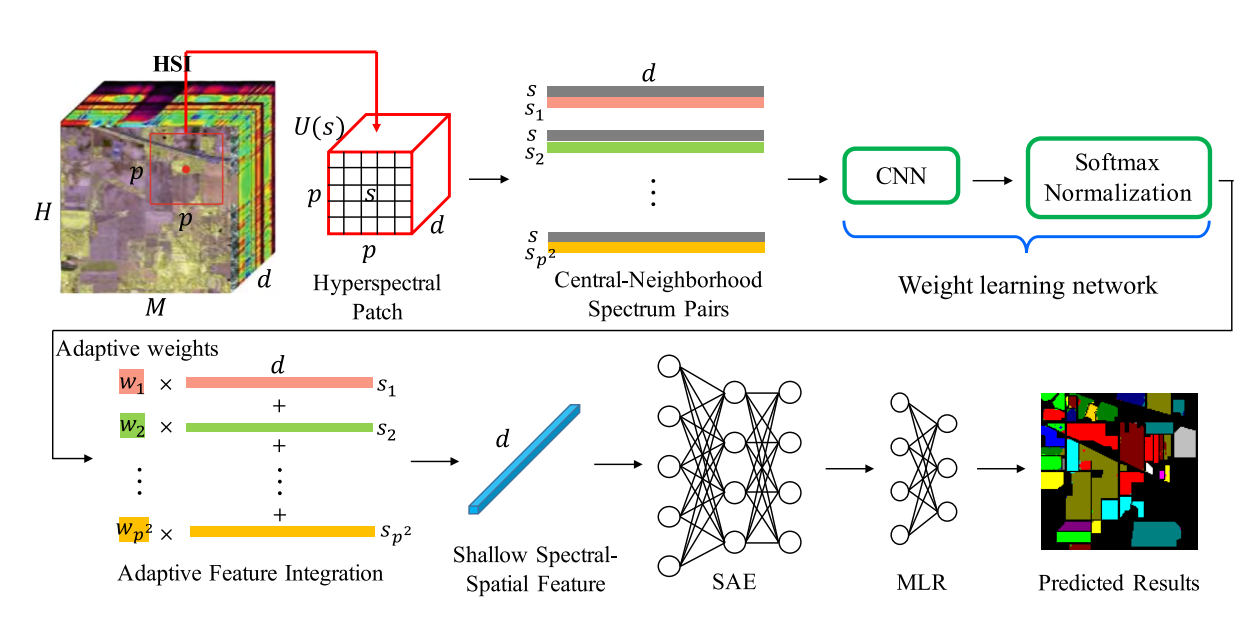
\includegraphics[width=1\textwidth]{Figures/assfln13.png}
  \caption{ASSFLN modelinin genel olarak çalışma şekli }
\end{figure}

\newpage
Bir başka bir yöntem ise. İlki hyperspectral görüntülerden tek tek pikselleri alıyor. Bu işlem için flat diye bir yöntem uyguluyor. Burada bahsedilen flat işlemi bu piksellerin birleştirmesini ifade ediyor. Sonra çıkardığı her bir pikselleri  başka bir yöntem olan pixel gömme olarak birleşitiryor.  Sonra BERT ismi verilen bir sıralı ağa veriyor. Bu işlemin ardından çıktıları tam-bağlı ağa verip burada eğittikten sonra sınıflandırma işlemi yapıyor \cite{he2019hsi}. Şekil 3.2'de anlatılan modelin görsel hali verilmiştir. \\

\begin{figure}[!ht]
  \centering
  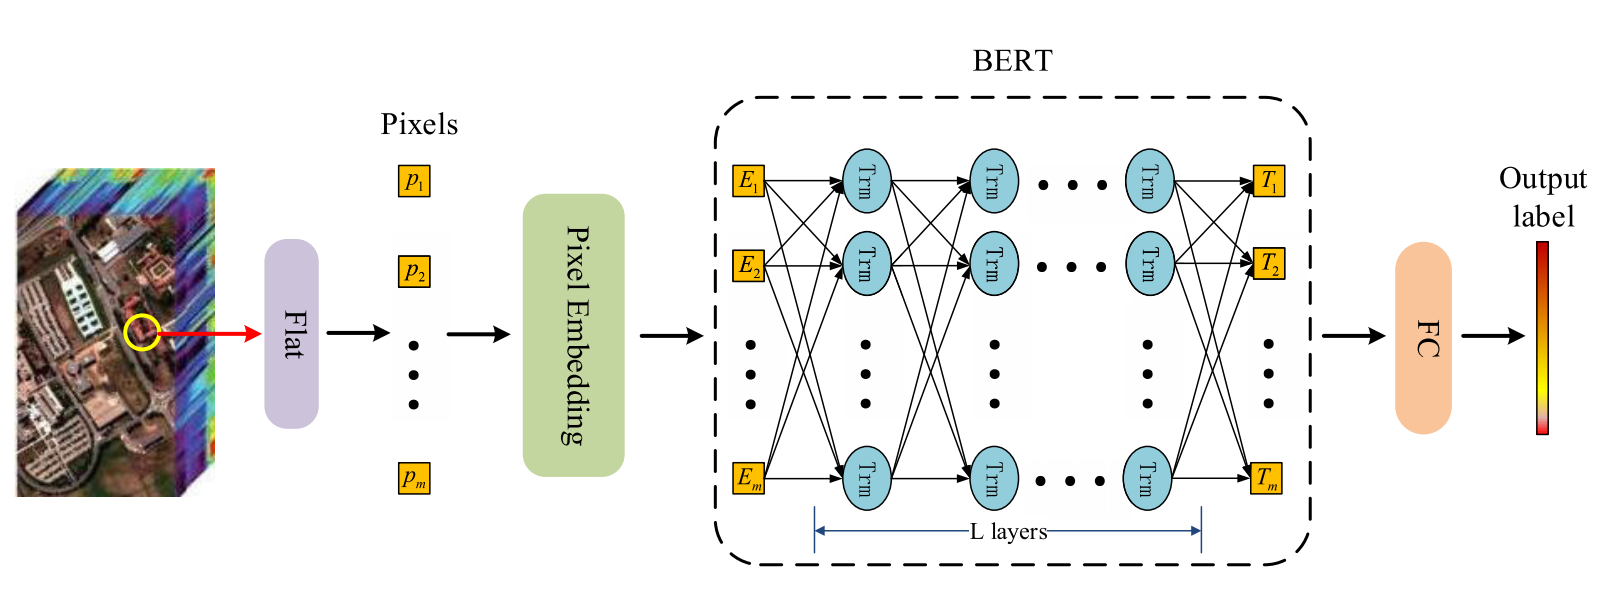
\includegraphics[width=1\textwidth]{Figures/bert14.png}
  \caption{BERT modelinin genel olarak çalışma şekli }
\end{figure}

\newpage
Yöntem temel olarak sınıflardan eşit örnek alınarak farklı ESA mimarilarinden oluşturulmuştur. Bu ESA mimarileri şunlardır; 3B-ESA, 2B-ESA,  D-3B ESA, D-2B ESA, D-Res-2B ESA, D-Res-3B-ESA mimarileri ile traning yapılıyor. Bunların çıktıları her birini bir vektör olarak hesaplıyor ve etkiket verileri ile arasında euclide uzaklığını hesaplıyor ve ardınan yitim( loss) fonksiyonuna veriyor. Danışmanlı özellikler(Supervised feature) çıkarıp Sinir Ağı(Neural Network) sınıflandırıcı ile sınıflandırıyor. Test amaçlı SVM ve bunun türevleri olan sınıflandırıca kulanılıyor fakat en iyi sonucu NN veriyor. Res olarak bahsedilen mimari son zamanlarda derin öğrenmede kullanılan residual olarak adı geçen yapıdır. Bir önceki ağdan gelen çıkıtıyı o anki ağdan çıkan çıktı ile toplama işlemi olarak kısaca anlatabiliriz \cite{roy2019hybridsn}. Şekil 3.3'de anlatılan modelin görsel hali verilmiştir. \\


\begin{figure}[!ht]
  \centering
  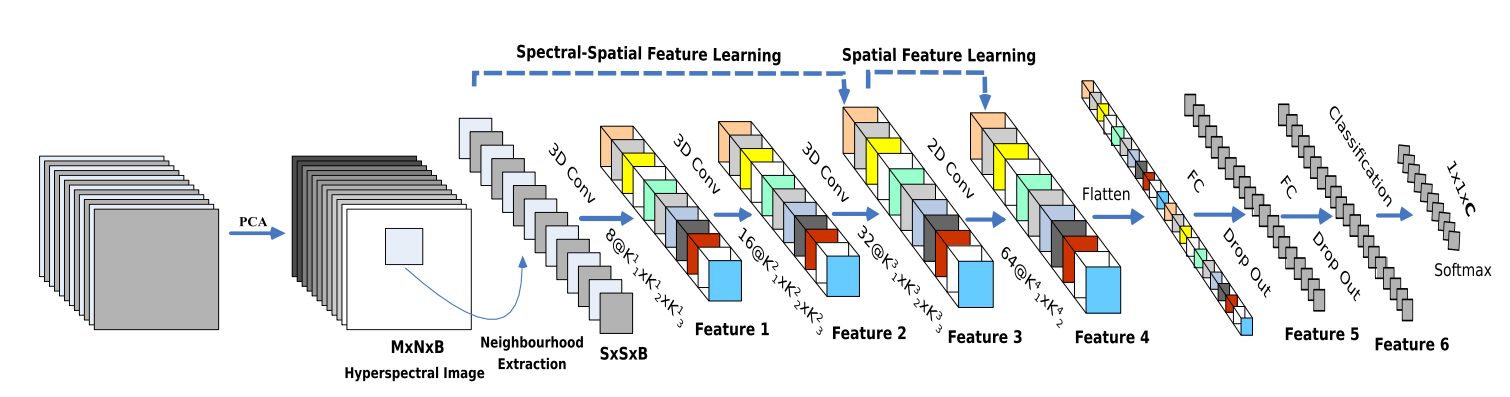
\includegraphics[width=1\textwidth]{Figures/hybrdidSN15.png}
  \caption{HybridSN modelinin genel olarak çalışma şekli }
\end{figure}

\newpage
Görüntü patchlere bölündükten sonra conv uygulanıp ardından pre-activation residual attention network yapılmıştır. Bunun amacı gradiant vanishing/explosing gibi problemleri önlemek ve sınıflandırma performansını arttırmak için yapmıştır. Sınıflandırma aşamasından önceği katman da ise global average pooling (GAP) kullanılmıştır ve daha sonra klasik sinir ağına verilip sınıflandırma yapılmıştır. Kayıp fonksiyonu olarak cross entropy loss kullanılmıştır. Residual blokları için relu kullanılmıştır. Son katman çıkışı olarak da sigmoid kullanılmıştır \cite{gao2019hyperspectral}.Şekil 3.4'de anlatılan modelin görsel hali verilmiştir. \\

\begin{figure}[!ht]
  \centering
  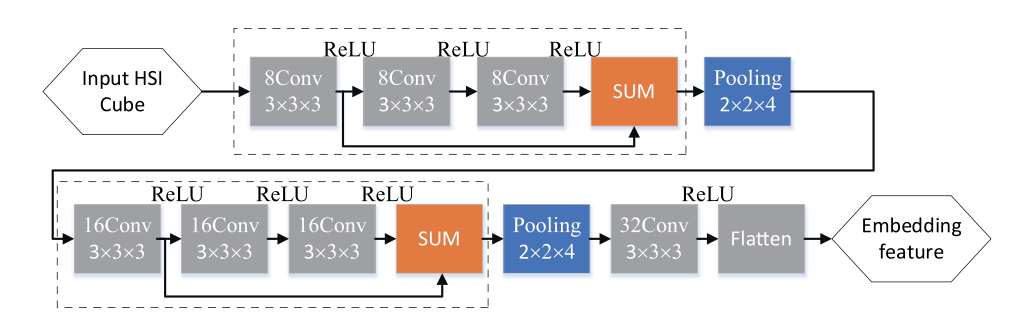
\includegraphics[width=1\textwidth]{Figures/gao16.png}
  \caption{GAO modelinin genel olarak çalışma şekli }
\end{figure}
\newpage
Giriş görüntüleri patchlere bölünüyor preporcessing olarak. Daha sonra spectral feature extraction için Evrişim 1*1 ve ReLU uygulanıyor.Bu işlemin ardından çoklu spectral-spatial feature learning işlemleri yapılıyor. Yanda görsel olarak verildiği gibi. Bu aşamadan sonra concatenated yapılıp feature fusion yaparak devam ediyor. Çıkış katmanında ise softmax kullanıyor \cite{bai2019ssdc}. Şekil 3.5'de anlatılan modelin görsel hali verilmiştir. \\

\begin{figure}[!ht]
  \centering
  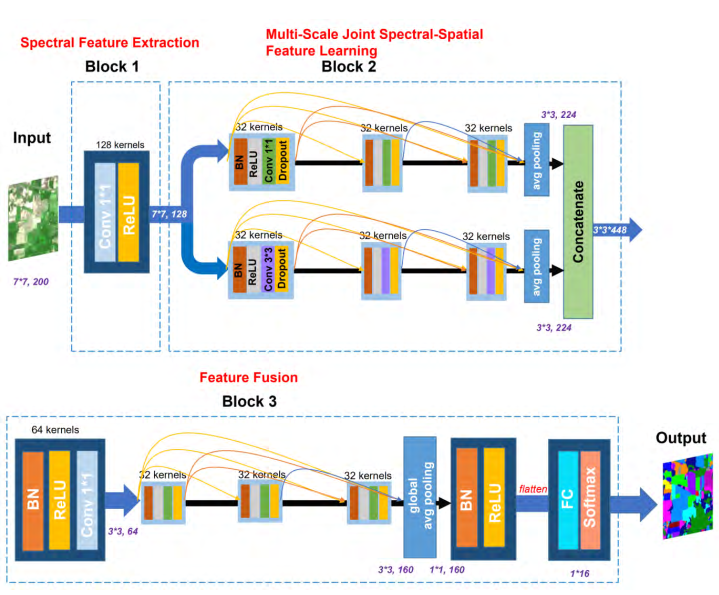
\includegraphics[width=1\textwidth]{Figures/ssfl17.png}
  \caption{SSDC-DenseNet modelinin genel olarak çalışma şekli }
\end{figure}

\newpage
İki aşamalı bir modeldir. İlk aşamada samples extranctions , yani örneklerden özellik çıkarma işlemi yapılıyor. Sonra 3B-SRNet  ağı ile özellik çıkarımı ve sınıflandırma işlemi yapıyor \cite{jiang2019hyperspectral}. Şekil 3.6'de anlatılan modelin görsel hali verilmiştir. \\

\begin{figure}[!ht]
  \centering
  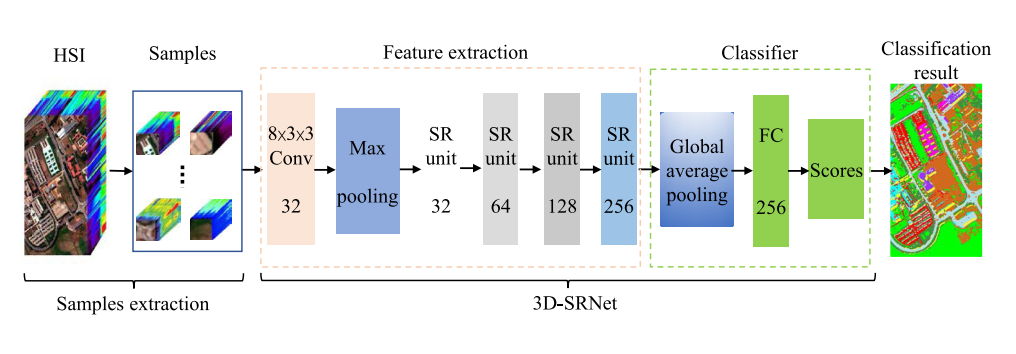
\includegraphics[width=1\textwidth]{Figures/3Dsrnet18.png}
  \caption{3D-SRNet modelinin genel olarak çalışma şekli }
\end{figure}
















\chapter{Konuyla İlgili Çalışmalar}

Giriş ve Motivasyon: Uzaktan algılama verilerini kullanan hava sahnesi sınıflandırması, verilerin özelliklerinden dolayı (az sayıda etiketli veri bulunması ve yüksek boyutluluk) hem askeri hem de sivil alanlarda en zorlu araştırma alanlarından biridir \cite{li2018deep}.Hiperspektral görüntü küpleri, farklı elektromanyetik spektrumlardan (spektral bantlardan) alınan yüzlerce veya binlerce uzamsal görüntüden oluşur. Bu nedenle, araştırma yapanlara aynı anda hem uzamsal hem de spektral bilgi sunarlar. Hiperpektral görüntülerin spektral çözünürlüğü yüksektir. Çünkü elektromanyetik spektrumdan (10-20 nm) dar bantlarda görüntüler almaktadır. Hiperspektral görüntülemede teknolojinin gelişmesiyle birçok ülke bu alana odaklanmıştır. Örneğin, Almanya’nın Environmental Mapping and Analysis Programı (EnMAP), Dünya'nın çevresini küresel ölçekte izlemeyi ve nitelendirmeyi hedeflemektedir. Bu durum günden güne uzaktan algılama görüntülerindeki artışa paralel olarak hiperspektral veri ambarlarında artışa neden olmaktadır. Bunun sonucunda da, görüntülerdeki gizli bilgilerin açığa çıkarılabilmesine imkân tanınmaktadır. Ancak, bu bilgilerin nasıl kullanılacağı daha fazla araştırma gerektiren açık bir konudur. Son yıllarda, birçok gerçek dünya örüntü tanıma uygulaması -özellikle yer bilimi ve uzaktan algılama alanında-, klasik makine öğrenme araçlarına kıyasla (ham veriden etkin özellik çıkartabilme yeteneğinden kaynaklanan) üstün performansı nedeniyle derin öğrenme tekniklerine büyük ilgi göstermektedir. “Derin öğrenme, çok sayıda doğrusal olmayan dönüşümlerden oluşan mimarileri kullanarak verilerde üst düzey soyutlamaları modelleyen bir dizi makine öğrenme algoritmasıdır”\cite{yan2018application}.Adından da anlaşılacağı gibi, Derin Sinir ağları hiyerarşik olarak düzenlenmiş birden fazla gizli katmana sahiptir. Ön katmanlarda basit bilgiler (kenarlar gibi) çıkarılmakta ve sonraki seviyelere iletilmektedir. Bu şekilde, sonraki seviyeler orta seviye bilgileri çıkarmaktadır. Bu işlem (bazı bilgileri girdi olarak alıp çıkış katmanında daha karmaşık bilgileri çıkartma) ağ hiyerarşisi sonuna kadar tekrar eder.\\
\newpage
	Özellikle, Evrişimli Sinir Ağları (Convolutional Neural Networks = CNN) \cite{lecun1998gradient} birçok bilgisayarlı görme problemi için güçlü bir araçtır. Diğer derin öğrenme algoritmalarından farklı olarak, CNN'ler, katlama – evrişim- (filtreleme) işleminin görüntünün belirli bir alıcı alanı (receptive field) üzerinde gerçekleştirildiği evrişim katmanlarını içerir. Derin Öğrenme mimarileri uzaktan algılamada birçok amaç için kullanılabilir: görüntü ön işleme, piksel tabanlı sınıflandırma, hedef tanıma, anlamsal özellik çıkarma ve sahne anlamlandırma. Derin Öğrenmenin uzaktan algılama verilerinde kullanımı bazı nedenlerden dolayı ekstra motivasyona sahiptir: 1) Uzaktan algılama verileri (özellikle çok bantlı ve hiperspektral görüntüler), çoklu spektral bantlar içerir. Bu, birkaç görüntüde bile veri miktarının çok büyük olduğu anlamına gelir. Bu yüzden daha fazla nörona ve daha derin sinir ağlarına ihtiyaç duymaktadır \cite{chen2013aircraft}. 2) Uzaktan algılama görüntüleri, doğal sahne görüntülerinden daha karmaşıktır. Farklı renk, konum, boyut ve yönelime sahip çeşitli nesne türlerinden oluşabilir. Bu karmaşıklık, doğal (natural) görüntü tanıma için ortak bir yaklaşım olan transfer öğrenmenin başarılı bir şekilde uygulanmasına engel olur. Transfer öğrenmede, derin öğrenme modeli çok sayıda etiketli numuneye sahip olan bir veri seti ile (ImageNet gibi) ön eğitimden geçirilmiştir. Ardından, sınırlı eğitim numuneleriyle sadece modelin son 2 veya 3 tam bağlı katmanını yeniden eğitilerek (önceki katmanlar değil) model parametreleri (ağırlıklar) güncellenir. Ayrıca, görsel farklılıklara 4 neden olan farklı sensörlerle görüntüler çekilebilir. 3) Her ne kadar derin öğrenme yöntemleri çok sayıda etiketlenmiş veri ile mükemmel bir performans sergilese de, uzaktan algılamada yalnızca sınırlı sayıda etiketli veri bulunmaktadır. Bu durum derin öğrenme yöntemlerinin performansını sınırlamaktadır. Yukarıda belirtilen nedenlerden ötürü, hiperspektral uzaktan algılama için en uygun derin sinir ağı mimarisinin geliştirilmesi zorlayıcı ve popüler bir araştırma alanıdır.\\
	
	Son zamanlarda, derin öğrenmenin doğal görüntü işleme alanındaki başarısını takiben, bu yöntemler HSI (Hyper-spectral Imaging = Hiperspektral görüntüleme) sınıflamasına da uygulanmış ve etkileyici sonuçlar elde edilmiştir \cite{chen2016deep} \cite{chen2015spectral} \cite{samaniego2008supervised}. Bu yaklaşımlar sırasıyla spektral bilgiden, uzamsal bilgiden ve spektral-uzamsal bilgiden faydalananlar olarak üç ana kategoride ele alınabilir. Uzamsal çözünürlük ile karşılaştırıldığında, spektral çözünürlük nispeten daha yüksektir. Her bir pikselden bir spektral vektör çıkarılabilir ve bu uzamsal piksele gömülü bilgi içeriğini tanımlamak için kullanılır. Geleneksel HSI sınıflandırma yaklaşımları yalnızca spektral bilgileri kullanır. Tipik sınıflandırıcılar arasında k-en yakın komşuluk \cite{samaniego2008supervised}, uzaklık ölçütü \cite{du2001linear}, lojistik regresyon \cite{li2010semisupervised}, ve en büyük olabilirlik kriteri \cite{ediriwickrema1997hierarchical} temelinde uygulanmış olanlar yer almaktadır. Her pikseli doğrudan spektral vektör üzerinden sınıflandırmak çoğu zaman makul ve verimli değildir. \\
	
	Literatürdeki geleneksel HSI sınıflandırma yaklaşımlarında, sınıflandırmayı desteklemek için özellik çıkarma yöntemleri de uygulanmıştır. Uzamsal özellikler genellikle tek bantlı bir görüntüden elde edilir. Günümüzde, uzamsal özellikler yaygın olarak 2D görüntü tarzında çalışan geleneksel Evrişimli Sinir Ağları (örneğin AlexNet \cite{NIPS2012_c399862d}, GoogLeNet \cite{szegedy2015going}, ResNet \cite{he2016deep} ile çıkarılmaktadır. Bununla birlikte, hiperspektral  görüntülerde kullanılan bantların sayısı çok yüksek olduğundan, işlemci teknolojisi gelişmiş olsa bile, bir bütün olarak 2D Evrişimli Sinir Ağlarına (CNN) bir girdi olarak verilemez. Bu nedenle, genellikle minimal 1D CNN mimarileri (evrişim katmanı + havuz katmanı + tam bağlı katman) \cite{hu2015deep} spektral özellik çıkarımı için kullanılır. Ayrıca, hesaplama maliyetini azaltmak ve ağ eğitimini geliştirmek için literatürde dropout ve batch normalization \cite{xu2014regression} teknikleri kullanılmaktadır. Giriş görüntülerini 1D vektörler olarak alan danışmansız derin öğrenme yaklaşımları (örneğin stacked auto encoders ve deep belief networks gibi) aynı zamanda temsil yeteneği olan spektral özellikleri ortaya çıkarmak için de kullanılır. Uzamsal ve spektral özelliklerin 2D ve 1D derin öğrenme mimarilerinden ayrı olarak çıkarılması, son işlem olarak bir birleştirme (fusion) stratejisi gerektirir.
	Bu doğrultuda ilk çalışma \cite{chen2014deep}, yazarların derin spektral özelliği çıkarmak için bir SAE (stacked auto encoder) kullandığı çalışmadır. Bu orijinal çalışmanın ardından, SAE yerine DBN (Deep Belief Network) kullanımı bildirilmiştir \cite{chen2015spectral}. Benzer şekilde, \cite{ma2016hyperspectral} nolu çalışma etkin özelliği öğrenmek ve ince ayar işleminde önsel göreceli bir mesafe eklemek için SAE'yi kullanmıştır.\\
	
Böylece yeterli sayıda etiketli örnek olmadığında istenen özelliklere ilişkin daha etkin bir
yönlendirme sağlanmıştır. \cite{xing2016stacked}, güçlü spektral özellikleri ayıklamak ve sınıflandırma işlemini tamamlamak için stacked denoising auto encoder ağını \cite{vincent2010stacked} kullanmıştır. Benzer bir fikir \cite{he2016hyperspectral} nolu çalışmada benimsenmiştir. Burada, HSI, deep stacking network (DSN) adı verilen yeni bir model ile sınıflandırılmıştır. Bir DSN modeli, her biri bir giriş katmanı, gizli 5 katman ve bir çıkış katmanı içeren birçok basit modülü içerir. Burada giriş katmanından gizli katmana ağırlıklar rasgele veya kontrastlı sapmalarla \cite{hinton2002training}, gizli katmandan çıkış katmanına ise yalancı ters alma işlemi ile başlatımlanır. Zhong vd. \cite{zhong2016diversified} HSI'daki sınıflandırma verimliliğini artırmaya yardımcı olan DBN'nin ön eğitim ve ince ayar işlemlerinde eğitim hedefinin optimizasyonuna çeşitliliği teşvik edici koşulları dâhil etmiştir.\\

	Yukarıda açıklanan spektral özellik çıkartma yöntemleri sadece spektral bilgileri kullanır ve uzamsal bilgileri kullanmaz. Oysa uzamsal bilgi, görüntüdeki komşu pikseller arasında ani bir değişiklik olmadığı hipotezine dayanmaktadır. Bu amaçla, ön işleme olarak, spektral bantları azaltmak için Temel Bileşen Analizi tekniği kullanılır. Daha sonra, derin spektral / uzamsal özellikler elde etmek için tüm hiperspektral görüntü küpüne 2D CNN uygulanır \cite{liang2016hyperspectral}.\\
	
Diğer bir yeni çalışma \cite{li2017hyperspectral} nolu çalışmada önerilmiştir. Burada, uzamsal özellikleri genişletmek için, derin CNN kullanımına dayalı HSI yeniden yapılandırma modeli önerilmiştir. Benzer fikirle, \cite{chen2014deep} ve \cite{lin2013spectral} nolu çalışmalarda PCA, HSI görüntülerinin boyutsallığını azaltmak için kullanılır. Ortaya çıkan veri küpleri tek boyuta indirgenir veya komşu bölgelerden çıkarılır. Bunu daha sonra, sınıflandırma işlemini gerçekleştiren bir SAE izler. \\

	Temel derin öğrenme modelleri (SAE, CNN ve DBN) dışında, son zamanlarda sıralı verilerden yararlanan Recurrent Neural Networks (RNN) de spektral bantların sürekliliğini modellemek için hiperspektral görüntü sınıflandırmasında kullanılmaktadır.
	Piksel tabanlı sınıflandırma yaklaşımlarından ayrı olarak, bir başka bakış açısı da bütün görüntüyü yerel görüntü patch’lerine bölmek ve her bir patch’i önceden tanımlanmış semantik
etiketlerden birine (endüstriyel alan veya yerleşim alanı gibi) atamaktır. Bu top-down yaklaşım genellikle sahne sınıflandırması olarak adlandırılır. Günümüzde bu sınıflandırma yaklaşımı, derin öğrenme mimarileri ile birlikte kullanılmaktadır. 

\chapter{Sonuçlar}

Geliştirmiş olduğumuz 3B-ESA-VAE modeli iyi sonuçlar üretmiştir.
Bu model Indian Pines ve Salinas veriseti üzerinde test edilmiştir. Doğruluk değerleri çeşitli
hiper parametlere göre değişmektedir. Bunun sebebi ise hızlı öğrenim yapması, aşırı öğrenme vb. olarak 
söyleyebiliriz.

\vspace{3cm}
% Side by side figures 
\begin{figure}[!ht]
    \begin{minipage}[c]{0.4\linewidth}
        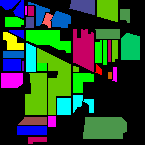
\includegraphics[width=0.7\textwidth]{Figures/IP_ground_.png}
        \caption{Indian Pines hedef sınıflandırma görüntüsü }
        \end{minipage}
    \hfill
        \begin{minipage}[c]{0.4\linewidth}
        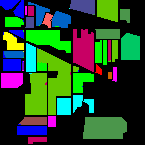
\includegraphics[width=0.7\textwidth]{Figures/IP_predicted_.png}
        \caption{Indian Pines tahmin sonucu oluşan çıktı }
    \end{minipage}%
\end{figure}

\begin{figure}[!ht]
    \begin{minipage}[c]{0.4\linewidth}
        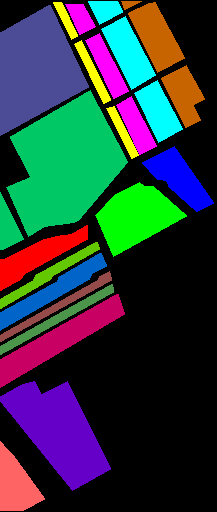
\includegraphics[width=0.7\textwidth]{Figures/SA_ground_.png}
        \caption{Salinas orjinal hedef sınıflandırma görüntüsü }
        \end{minipage}
    \hfill
        \begin{minipage}[c]{0.4\linewidth}
        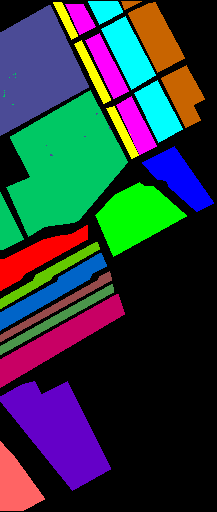
\includegraphics[width=0.7\textwidth]{Figures/SA_predicted_.png}
        \caption{Salinas tahmin sonucu oluşan çıktı }
    \end{minipage}%
\end{figure}
\newpage

\vspace{2cm}
\begin{table}[!ht]
\centering
    \begin{threeparttable} % <--- new
    \caption{Sonuçların sayısal değeleri}
        \begin{tabular}{|c|c|c|c|}
        \hline
        \textbf{Veriseti Adı} & \textbf{Kappa(\%)} & \textbf{Ortalama Doğruluk} & \textbf{Genel Doğruluk} \\ \hline
        Indian Pines & 0.989    & 99.038           & 99.038         \\ \hline
        Salinas & 0.999    & 99.881          & 99.881         \\ \hline
        \end{tabular}
    \end{threeparttable} % <--- new
\end{table}

Geliştirmiş olduğumuz modelin Tablo 5.1'de Şekil 5.2 ve Şekil 5.4 resimlerin orjinal resim ile karşılaştırmasının sayısal sonuçları verilmiştir.


%%%%%%%%%%%%%%%%%%%%%%%%%

%%%%% References %%%%%%%%%%%%%
\setstretch{1}
\printbibliography[heading=bibnumbered, title={\bibName}]
%%%%%%%%%%%%%%%%%%%%%%%%%


\end{document}
